\documentclass[12pt]{ut-thesis}

% ----------------------------------------------------------------------------------------------------------------------------------------
% USEPACKAGE DECLARATIONS
% ----------------------------------------------------------------------------------------------------------------------------------------

%\includeonly{./sections/reionization}

\usepackage{amsmath}
\usepackage{amssymb}
\usepackage{aas_macros}
\usepackage{natbib}
\usepackage{html}
\usepackage{graphicx}
\usepackage{rotating}
\usepackage{tabularx}
\usepackage{pdflscape}
\usepackage{afterpage}
\usepackage{capt-of}
\usepackage{setspace}
\doublespacing 


%\usepackage[figuresleft]{rotating}

% ----------------------------------------------------------------------------------------------------------------------------------------
% AUTHOR INFORMATION
% ----------------------------------------------------------------------------------------------------------------------------------------

\degree{Doctor of Philosophy}
\department{Astronomy and Astrophysics}
\gradyear{2016}
\author{Liam Dean Connor}
\title{Long Wavelength Astrophysics}

% ----------------------------------------------------------------------------------------------------------------------------------------
% COMMANDS AND DEFINITIONS
% ----------------------------------------------------------------------------------------------------------------------------------------

% Put here all other formatting commands that belong in the preamble. In particular, you should put all of 
% your \newcommand's, \newenvironment's, \newtheorem's, etc. (in other words, all the global definitions 
% that you will need throughout your thesis) in a separate file and use "\input{filename}" to input it here.
\input{commands}

% Table of contentds depth (0 = chapter, 1 = section, 2 = subsection, 3 = subsubsection, etc.)
\setcounter{tocdepth}{2}

% Make each page fill up the entire page.
\flushbottom

% ==============================================================================
% PRELIMINARY CONTENT
% ==============================================================================

\begin{document}

% This sets the page style and numbering for preliminary sections.
\begin{preliminary}

% This generates the title page from the information given above.
\maketitle

% There should be NOTHING between the title page and abstract.  However, if your document 
% is two-sided and you want the abstract _not_ to appear on the back of the title page, then uncomment 
% the following line.
% \cleardoublepage

% ----------------------------------------------------------------------------------------------------------------------------------------
% ABSTRACT
% ----------------------------------------------------------------------------------------------------------------------------------------

\begin{abstract} % At most 350 words for Ph.D.

\end{abstract}

% Anything placed between the abstract and table of contents will appear on a separate page since the 
% abstract ends with \newpage and the table of contents starts with \clearpage.  Use \cleardoublepage
% for anything that you want to appear on a right-hand page.

% ----------------------------------------------------------------------------------------------------------------------------------------
% DEDICATION
% ----------------------------------------------------------------------------------------------------------------------------------------

%\begin{dedication}
\vspace*{\fill}
\begin{center}
{\em }%To Pop and my infinitely supportive parents}
\end{center}
\vfill
%\end{dedication}

\newpage % Force separate pages for dedication and acknowledgements


% ----------------------------------------------------------------------------------------------------------------------------------------
% ACKNOWLEDGEMENTS
% ----------------------------------------------------------------------------------------------------------------------------------------

\begin{acknowledgements}
 % The research presented in this thesis sample the work 
 % I have done over the last five years, which has 
 % ranged from what felt like mathematical musings to software development  
 % to on-site hardware work. This is because both of my supervisors, 
 % Ue-Li Pen and Keith Vanderlinde, possess end-to-end expertise, 
 % with firm understanding of the physics in which we are interested 
 % as well as the steps required to make such measurements come to fruition;
 % needless to say this thesis would not have been possible without them. 
 % A similarly insightful supervisory figure was Richard Shaw, 
 % whose ease with signal processing, statistics, and computing 
 % was greatly appreciated in my first few years of graduate school. 

 % On the CHIME team, I was lucky enough to work closely 
 % with such world-class experimental cosmologists as Mark Halpern 
 % and Gary Hinshaw. Tom Landecker was an irreplaceable source 
 % of knowledge and wisdom during my many 
 % visits to DRAO, acting as the token radio astronomer in a 
 % large radio astronomy project. I would also thank my 
 % thesis committee, including Barth Netterfield and Mike Reid. 

\end{acknowledgements}

% ----------------------------------------------------------------------------------------------------------------------------------------
% TABLE OF CONTENTS
% ----------------------------------------------------------------------------------------------------------------------------------------

\tableofcontents

% ----------------------------------------------------------------------------------------------------------------------------------------
% LIST OF TABLES
% ----------------------------------------------------------------------------------------------------------------------------------------

\listoftables

% ----------------------------------------------------------------------------------------------------------------------------------------
% LIST OF FIGURES
% ----------------------------------------------------------------------------------------------------------------------------------------

%\listoffigures

\end{preliminary}

% ==============================================================================
% CHAPTERS
% ==============================================================================

%%%%%%%%%%%%%%%%%%%%%%%%%%%%%%%%%%%%%%%%%%%%%%%%%%%%%%%%%%%%%%%%%%%%%%%%
%%  Put your Chapters here; the easiest way to do this is to keep     %%
%%  each chapter in a separate file and `\include' all the files.     %%
%%  Each chapter file should start with "\chapter{ChapterName}".      %%
%%  Note that using `\include' instead of `\input' will make each     %%
%%  chapter start on a new page, and allow you to format only parts   %%
%%  of your thesis at a time by using `\includeonly'.                 %%
%%%%%%%%%%%%%%%%%%%%%%%%%%%%%%%%%%%%%%%%%%%%%%%%%%%%%%%%%%%%%%%%%%%%%%%%

\include{./sections/introduction}
% \include{./sections/chime}
% \chapter{Beamforming}
\label{chapter:beamforming}
\chaptermark{Relative velocity reconstruction}



% ================================================================================
% CHAPTER OVERVIEW
% ================================================================================

\section{Chapter Overview}

Beamforming
% ================================================================================
% INTRODUCTION
% ================================================================================

\section{Introduction}


  
% ================================================================================
% THEORY AND IMPLEMENTATION
% ================================================================================
  
\section{Theory and Implementation}
\label{sec:theory}

Beamforming is a signal processing technique that allows for 
spatial filtering, and has greatly benefited a diverse set of fields 
from radar and wireless communications to radio astronomy. % Insert history

By coherently combining the voltages of a multi-element array, 
sensitivity can be allocated to small regions of the sky and 
the array's effective forward gain can be increased. The signal 
from each antenna, $x_n$, is multiplied by a complex weight, whose 
phases, $\phi_n$, are chosen to destructively interfere the radio waves 
in all directions but the desired pointing. The signals 
from all antennas are then combined to give the formed beam 
voltage stream, $X_{\rm BF}$.

\begin{equation}
\label{eq-bf_sum}
X_{\rm BF} = \sum_{n=1}^N a_n e^{i\phi_n} x_n
\end{equation}

\noindent Here $a_n$ are real numbers that can be used to as 
amplitude weightings for the antennas. If we define a more 
general complex weighting, $w_n \equiv a_n e^{i\phi}$, and 
switch to vector notation, Eq.~\ref{eq-bf_sum} becomes,



\begin{align}
\rm{sin}(alt) = \rm{sin}(\delta)\, \rm{sin}(lat) + cos(\delta)\, cos(lat)\, cos(\rm HA)\\
\rm{cos}(az) = \frac{\rm{sin}\delta - \rm{sin}(alt) \,
\rm{sin}(lat)}{\rm{cos}(alt)\, \rm{cos}(lat)}
\end{align}

\subsection{Neutrino $N$-body Particles in \cpm{}}
\label{}

We simulate a single neutrino species as an $N$-body particle. Initial neutrino positions are generated separately from CDM using the same Gaussian noise map. We use neutrino density transfer functions, $\tdel$, computed via \camb{} \citep{lewis/etal:2000} for a universe with one massive and two massless neutrinos. The initial neutrino velocity is composed of two parts: a linear component (analogous to the Zel'dovich velocity) plus a random thermal component.  For the linear component, we first compute the linear neutrino velocity transfer function, $\tvel$, via the continuity equation under the assumption that initial conditions are adiabatic and velocities are linear (e.g. $\delta(k,z) = \tdel(k,z) \delta_i(k)$ and $\vec{v}(\vec{k},z) = \tvel(k,z) \delta_i(k) \hat{k}$ for an initial perturbation $\delta_i(k)$):
\bq
\dot{\delta} + \frac{1}{a}\vec{\nabla}\cdot\vec{v} = 0 \rightarrow \tvel = - i \frac{H}{k} \frac{\tdel(z+\delta z) - \tdel(z-\delta z)}{2 \delta z},
\label{eq:veltransfer}
\eq
where we convert time derivatives to redshift derivatives and evaluate numerically using a spacing $\delta z = 0.1$. We have checked that the transfer functions computed via equation \ref{eq:veltransfer} are in good agreement with those produced by the {\small CLASS} code \citep{blas/etal:2011} in Newtonian gauge\footnote{The {\small CAMB} density transfer functions are in the synchronous gauge whereas the velocity transfer function we desire are in the longitudinal Newtonian gauge.  However, the gauge transformation terms are proportional to the time derivatives of the Newtonian potentials which we already ignore in the continuity equation.}.  
  
From this velocity transfer function, we compute a velocity potential, $\phi_v(k)$, such that $\vec{v}(k) = i \vec{k} \phi_v(k) = (\tvel/\tdel)\delta \hat{k}$. When combined with equation \ref{eq:veltransfer} this yields:
\bq
\phi_v(k) = - \frac{H}{k} \frac{\tdel(z+\delta z) - \tdel(z-\delta z)}{2 \delta z} \frac{\delta}{\tdel}.
\label{eq:velpotential}
\eq
This potential is then Fourier transformed and a two-sided finite difference is taken to obtain the linear velocity.  Using a real-space gradient reduces the number of Fourier transforms to be computed and is consistent with our calculation of the displacement field.  

The random component of the velocity is computed via the
cumulative distribution function, ${\rm CDF}[v,\beta]$, which
follows from the relativistic Fermi-Dirac distribution,
${\rm PDF}[v,\beta]$, for neutrinos:
\bqa
{\rm PDF}[v,\beta] &= & \frac{1}{N}\left(\frac{m_\nu}{kT}\right)^3\frac{v^2}{e^{m_\nu v/kT}+1} = \frac{\beta^3}{N}\frac{v^2}{e^{v\beta}+1} \nonumber \\
{\rm CDF}[v, \beta] &=& \int_0^v {\rm PDF}[u,\beta] du \nonumber   \\
                              &=&\frac{1}{N} \int_0^{w=\beta v} \frac{w^2}{e^w+1}dw \nonumber \\
                              &=&{\rm CDF}[\beta v,1]
\label{eq:fermicdf}
\eqa
where $m_\nu$ and $T$ are neutrino mass and temperature, respectively, $\beta \equiv m_\nu/kT$ and $N = \int_0^\infty w^2/(e^w+1) dw \simeq 1.803$ is a normalization constant.  Our numerical evaluation of the $\rm CDF$ gives a maximum particle speed of $0.013 \left(0.2\:\ev/m_\nu\right) (1+z_i)c$ for a given starting redshift $z_i$.  Neutrinos in the mass regime we are interested in are relativistic at the redshift for which CDM initial conditions are generated ($z_c = 100$):
\bq
\langle v \rangle = \frac{\int_0^\infty v{\rm PDF}[v,\beta] dv}{\int_0^\infty {\rm PDF}[v,\beta] dv} \approx 800 \left(\frac{0.2\ \ev}{m_\nu}\right) (1+z)\ \kms.
\eq
This thermal motion would dominate the time step constraining the maximum distance a particle may travel, making the simulation impractically slow.  To circumvent this issue we evolve the CDM in isolation to a lower redshift, $z_\nu \sim 10$, at which point neutrinos are added and the two components evolve together.
  
During their subsequent evolution, CDM and neutrino particles are treated identically except for their masses, which are weighted by their energy fractions as well as number ratio:
\bq
m_i = \frac{\Omega_i}{\Omega_m}\frac{N_g}{N_i},
\label{eq:pmass}
\eq
where $\Omega_i$ is the energy fraction of species $i$, $\Omega_m$ is the total matter energy fraction, $N_g$ is the number of cells in the simulation grid, and $N_i$ is the number of particles of species $i$.  These masses are used when adding particles to the grid for the computation of the long-range gravitational force as well as the short-range pairwise force.  The particle type is distinguished within the code using 1 byte particle identification tags.  

\subsection{Density and Velocity Fields}
\label{ssec:velocity}

We compute CDM, neutrino, and halo density fields using a standard cloud-in-cell interpolation method for both CDM and neutrinos. Computing velocity fields from particle-based simulations has only recently been studied in depth. This may be related to the ambiguity associated with defining a velocity field from a sample of point particles. Unlike quantities such as mass or momentum, the velocity of a particle cannot be simply added to a grid. The most obvious method for generating a velocity field is to divide a gridded momentum field by its corresponding density field. However, within void regions it is possible that empty cells exist for which no well-defined velocity can be assigned. Alternatively, one may define the velocity at a given grid cell to be the average velocity of the $N_{\rm near}$ nearest particles about this point.  The application of the nearest particle method was studied by \citet{zhang/etal:2015} and \citet{zheng/etal:2015} where it was found that the velocity power is suppressed for low particle number densities, $n<1\ (\mpch)^{-3}$, due to the sampling procedure.  In our simulations we use high number densities, $n_{\rm dm} \sim 10\ (\mpch)^{-3}$, and therefore do not expect this effect to be significant.  More advanced methods for computing velocity fields exist such as phase-space interpolation discussed in \citet{pueblas/scoccimarro:2009} and more recently in \citet{hahn/etal:2014}.  The neutrino velocity distribution has been studied by \citet{villaescusa-navarro/etal:2013}.
  
In what follows we compute the velocity fields of CDM and neutrinos in different ways.  For CDM, we adopt the nearest particle method and take the $N_{\rm near} = 1$ nearest particle about the centre of each cell using the same grid resolution as neutrinos.  We have found that the nearest particle method can also be used for neutrinos albeit with a much larger $N_{\rm near} = 64$ to smooth the field on small scales. However, searching over this many particles is a computationally expensive task.  For neutrinos we therefore employ the approach of dividing their momentum field by their density field on grids coarsened so that there is always at least one neutrino per cell. This is possible since neutrinos are rather homogeneously distributed and form voids to a lesser extent than CDM.

We treat the velocity fields obtained from the nearest particle and momentum methods as faithful tracers of the actual field. However, these fields are not comparable to observational data since neither CDM nor neutrino velocities can be directly measured.  For this purpose we reconstruct velocity fields from density fields using linear theory:
\bq
\vec{v} = \frac{\tvel}{\tdel}\frac{\vec{k}}{k}\delta,
\label{eq:vrec}
\eq
where we use CDM and halo density fields separately for $\delta$ (although with the same $\tdel$).  In what follows we treat halos as point particles of unit mass in order to represent the information available through galaxy surveys.  
  
Poisson noise is a severe hindrance in computing neutrino statistics as the large thermal velocity causes neutrino particles to be more homogeneously distributed.  For density spectra it is possible to subtract out the flat Poisson noise spectrum but this is not possible for velocity fields.  Instead, we use a method that exploits the fact that Poisson noise arises from particles being randomly distributed.  The procedure for either density or velocity fields is:
\begin{enumerate}
\item Randomly divide the particles into two groups.
\item Interpolate particles of each group into a field (density or velocity).
\item Compute the cross spectrum between groups as an estimate of the auto spectrum.
\end{enumerate}
This procedure ensures that Poisson noise is highly suppressed as the noise between the two groups is uncorrelated due to the random assignment to groups.  We use this method for density and velocity auto-spectra for both CDM and neutrinos; we do not use it for CDM-neutrino cross spectra where it is redundant (there are already two groups of particles).  
  
The accuracy of the reconstructed field is measured using a correlation coefficient:
\bq
r_{ij}(k) = \frac{\Delta^2_{ij}(k)} { \sqrt{\Delta^2_{ii}(k)\Delta^2_{jj}(k)} }
\label{eq:rij} 
\eq
where $\Delta^2_{ij}$ is the cross power spectrum between species $i=c,h,\nu \textrm{ or rel}$ using reconstruction method $\mbox{sim}, \mbox{Rec DM}, \mbox{Rec HA}$ (nearest particle/momentum, equation \ref{eq:vrec} with CDM and equation \ref{eq:vrec} with haloes respectively) and species $j$ (with potentially a different reconstruction method).  We also define the integrated correlation coefficient as:
\bq
r_{ij} = \frac{\int \Delta^2_{ij} \frac{dk}{k}}{\sqrt{\int \Delta^2_{ii} \frac{dk}{k}} \sqrt{\int \Delta^2_{jj} \frac{dk}{k}}}
\label{eq:intrij}
\eq
which no longer depends on wavenumber.
  
% ================================================================================
% RESULTS
% ================================================================================  
  
\section{Results}
\label{sec:nu-results}

In this section we present the results for a suite of four simulations of CDM and neutrinos.  We simulate neutrinos of mass $m_\nu = 0.4, 0.2, 0.1$ and $0.05\:\ev{}$.  Each simulation contains $N_c = 1536^3$ CDM particles and $N_\nu = 3072^3$ neutrino particles within a periodic box of side length $L = 500\ \mpch$. In each case CDM is started from an initial redshift $z_c = 100$ and gravitational forces are softened below the scale $r_{\rm soft} = 24$ kpc/$h$.  Neutrinos are added in at redshift $10$ for all species except $0.05\:\ev{}$ which we add at redshift $5$.  We assume a base cosmology compatible with Planck results: $\Omega_b = 0.05$, $\Omega_c = 0.27$, $\sigma_8 = 0.83$, $n_s = 0.96$, $h = 0.67$, and compute
\bq
\Omega_{\nu} = \frac{m_\nu}{93.14\ h^2}
\label{eq:omnu}
\eq
as in \citet{mangano/etal:2015}. We hold $\Omega_b$ and $\Omega_c$ fixed in each simulation and maintain a flat universe by adjusting $\Omega_\Lambda = 1 - \Omega_m = 1 - \Omega_b - \Omega_c - \Omega_\nu$. In what follows we mainly investigate a fiducial simulation with $m_\nu = 0.2$ eV.  We label our simulations based on neutrino mass with S05, S1, S2, and S4 denoting the simulations with $m_\nu = 0.05, 0.1, 0.2$, and $0.4\:\ev{}$ respectively.  

Halo catalogues are generated for each simulation at $z = 0$ using a spherical overdensity algorithm that considers all halos with at least 100 CDM particles. This corresponds to a minimum halo mass of $3 \times 10^{11}\ M_\odot/h$. Recall, however, that we assign each halo unit mass when constructing halo density fields in order to emulate the information available in galaxy surveys. In what follows, density and velocity fields for CDM, neutrinos, and halos are computed on uniform rectilinear grids containing $1536^3$ mesh cells.  
    
\subsection{Density}
\label{ssec:density}

% -------------------------------------------- FIGURE 1 --------------------------------------------
\begin{figure}
\begin{center}
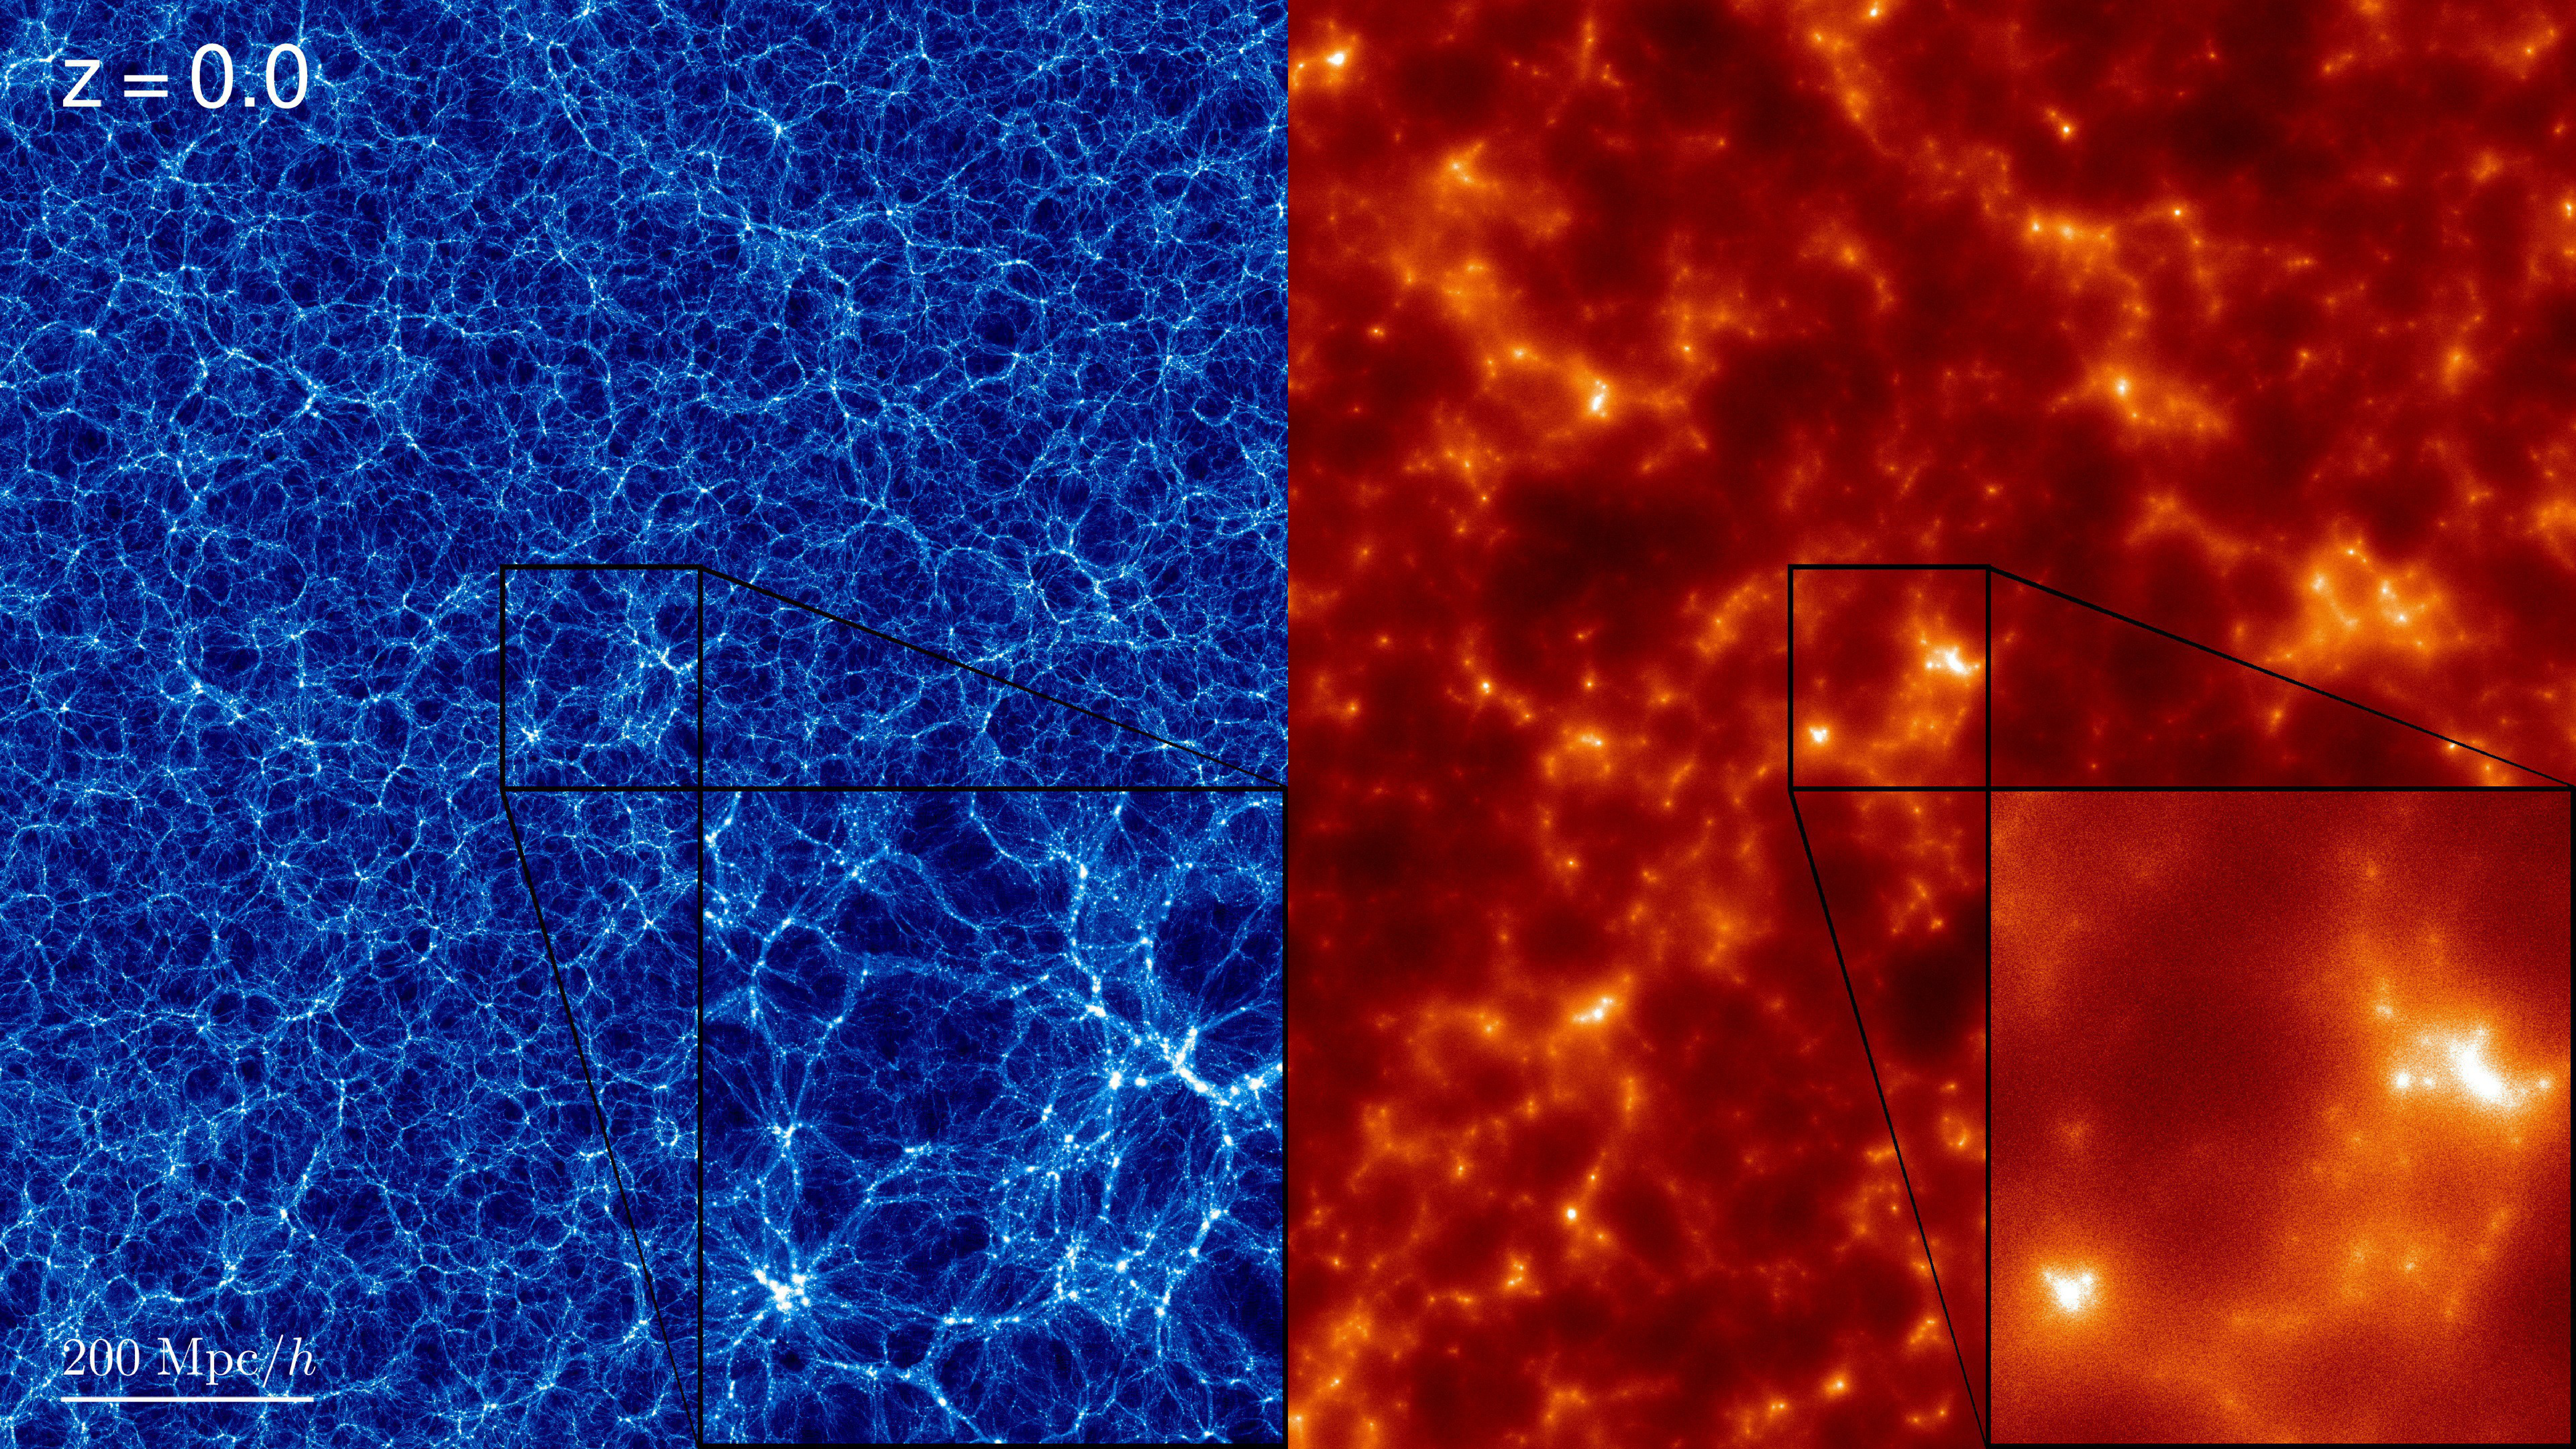
\includegraphics[width=0.85\textwidth]{./figures/neutrinos/fig1.pdf} \vspace{-0.1cm}
\caption[Cold dark matter, neutrino, and halo density slices]
{Density slices of equal width $500\ \mpch{}$ and
thickness $1.3\ \mpch{}$ from various simulations at
$z = 0$.  The top row shows cold dark matter (left) and halo
(right) density slices from the 0.2\ \ev{} neutrino
simulation. The middle row compares neutrino density slices
from the 0.05 (left) and 0.1 (right)\ \ev{} simulations
while the bottom row shows the 0.2 (left) and 0.4 (right)\
\ev{} simulations.  It is easy to see by eye that the cold dark
matter and neutrino density fields are highly correlated and
that heavier neutrinos cluster more than lighter ones.}
\vspace{-0.5cm}
\label{fig:denslice}
\end{center}
\end{figure}
% -------------------------------------------- FIGURE 1 --------------------------------------------

Figure \ref{fig:denslice} compares slices of the CDM and halo density fields at $z = 0$ from simulation S2 to the neutrino density fields from simulations S05, S1, S2, and S4.  It is easy to see that the neutrino density fields are correlated with the CDM density field albeit with much less clumping in the former than the latter as evidenced by their respective colour bars. In addition, we see that higher mass neutrinos tend to clump more than lower mass neutrinos as they are more influenced by the underlying CDM distribution due to their lower thermal velocities.

% -------------------------------------------- FIGURE 2 --------------------------------------------
\begin{figure}[!t]
\begin{center}
\includegraphics[width=\smwidth]{./figures/neutrinos/fig2.pdf} \vspace{-0.1cm}
\caption[Cold dark matter, neutrino, and halo density power spectra]
{The dimensionless matter power spectra at $z = 0$ for
cold dark matter (solid black line), halos (solid blue line)
and neutrinos (solid red line) from S2. Shot noise has been
removed by computing the cross-spectrum between two randomly
chosen groups for each species.  Also plotted are the linear
and nonlinear cold dark matter (dotted black and dashed
black lines) and neutrino (dotted red and dashed red lines)
power spectra. Note that there is a small numerical artifact
in the linear neutrino transfer function just above
$k = 1\:\hmpc$ that should be ignored.}
\vspace{-0.2cm}
\label{fig:denpow}
\end{center}
\end{figure}
% -------------------------------------------- FIGURE 2 --------------------------------------------

% -------------------------------------------- FIGURE 3 --------------------------------------------
\begin{figure}[!b]
\begin{center}
\includegraphics[width=\smwidth]{./figures/neutrinos/fig3.pdf} \vspace{-0.1cm}
\caption[Cold dark matter-neutrino cross correlation coefficient]
{The cold dark matter-neutrino cross correlation
coefficient at $z = 0$ from S2. As expected, neutrinos are
highly correlated with cold dark matter over a large range
of scales.}
\label{fig:dencorr}
\end{center}
\end{figure}
% -------------------------------------------- FIGURE 3 --------------------------------------------

Figure \ref{fig:denpow} shows the dimensionless power spectra for CDM, halos, and neutrinos at $z = 0$ from S2.  Also plotted are theoretical predictions for CDM and neutrinos, which are computed via
\bq
\Delta^2_i(k) = \frac{k^3}{2\pi^2}  P_m\left(\frac{T_i}{T_m}\right)^2,
\label{eq:PNL}
\eq    
where $T_i$ is the linear transfer function for species $i$, $T_m$ is the total matter linear transfer function, and $P_m$ is either the linear (computed from \camb{}) or the nonlinear [computed from \hfit{} \citep{smith/etal:2013}] total matter power spectrum. We first note that the group cross-correlation method we employ effectively removes the shot noise allowing us to understand statistical properties even of the noisy neutrino density field.  We find that the CDM power spectrum agrees well with the nonlinear prediction up to large $k$.  The neutrino power spectrum, on the other hand, is significantly enhanced on small scales compared to the theoretical curve demonstrating that the linear response of equation \ref{eq:PNL} fails to capture neutrino dynamics on small scales.  This trend was previously observed by Ali-Ha{\"i}moud (private communication) and modelled in \citet{massara/etal:2014}.

Despite their enhanced power on small scales, neutrinos remain highly correlated with the CDM density field, as was qualitatively discussed with Figure \ref{fig:denpow}.  More quantitatively, Figure \ref{fig:dencorr} shows the $z = 0$ cross-correlation coefficient between CDM and neutrinos from S2 as a function of wavenumber. We find that neutrinos exhibit $r_{c\nu} \gtrsim 0.9$ correlation with CDM on all scales $k < 1\ \hmpc$ and achieve $r_{c\nu} \sim 0.85$ down to the smallest scales resolved in the simulation.

The halo power spectrum is also plotted in Figure \ref{fig:denpow}. As expected, the halo power follows the general shape of the CDM power spectrum, but with a reduced amplitude, or bias.  We define the bias as:
\bq
b \equiv \sqrt{\frac{P_{hh}}{P_{cc}}},
\label{eq:bias}
\eq
and plot it as a function of $k$ in Figure \ref{fig:denbias}. Defining the bias with respect to the CDM power spectrum instead of the total matter spectrum (e.g. including neutrinos) was shown to be less scale dependent in \citet{castorina/etal:2014}. The bias is roughly constant on large scales with $b \sim 0.8$ and falls off on small scales as the halo density field does not include contributions from the ``one-halo'' term describing the internal mass profile of halos \citep{scherrer/bertschinger:1991}. Hence, halo power is suppressed on scales comparable to the typical virial radii of halos which occurs at $k \sim 0.2\ h/{\rm Mpc}$ for the largest halos in the box.

% -------------------------------------------- FIGURE 4 --------------------------------------------
\begin{figure}[!t]
\begin{center}
\includegraphics[width=\smwidth]{./figures/neutrinos/fig4.pdf} \vspace{-0.1cm}
\caption[Halo bias scale dependence]
{The halo bias parameter measured from S2 at $z = 0$.
On scales $k \lesssim 0.2\ h/{\rm Mpc}$ the bias is roughly
constant with $b \sim 0.8$. The bias falls off on smaller
scales as power is suppressed within the typical virial
radii of halos.}
\vspace{-0.2cm}
\label{fig:denbias}
\end{center}
\end{figure}
% -------------------------------------------- FIGURE 4 --------------------------------------------

\subsection{Velocity}

Figure \ref{fig:velslice} compares slices of CDM, neutrino, and CDM-neutrino relative velocity computed from the simulation particles as well as reconstructed from the CDM and halo density fields using equation (\ref{eq:vrec}). We observe a similar trend as the density fields with CDM and neutrinos highly correlated in velocity. In addition, we see that the velocity fields reconstructed from only knowledge of either the CDM or halo density field qualitatively agree with the large-scale structure of the velocity fields obtained within the simulation.

% -------------------------------------------- FIGURE 5 --------------------------------------------
\begin{figure}
\begin{center}
\includegraphics[width=0.99\textwidth]{./figures/neutrinos/fig5.pdf} \vspace{-0.1cm}
\caption[Slices of simulated and reconstructed velocity fields]
{Slices of equal width $500\ \mpch{}$ and thickness
$1.3\ \mpch{}$ showing the $z = 0$ velocity component
perpendicular to the page for cold dark matter (top row),
neutrinos (middle row), and the relative velocity between
cold dark matter and neutrinos (bottom row). Columns show
the velocity fields from the simulation particles (left
column), reconstructed from the cold dark matter density
field (middle column), and reconstructed from the halo
density field (right column). We see that both of the
reconstruction methods agree well with the large-scale
structure of the simulation velocity fields.}
\vspace{-0.5cm}
\label{fig:velslice}
\end{center}
\end{figure}
% -------------------------------------------- FIGURE 5 --------------------------------------------

Figure \ref{fig:velpow} compares the simulated CDM and neutrino velocity power spectra to the CDM and halo reconstructed fields. Note that for the latter we take $\delta = \delta_h/b$ in equation (\ref{eq:vrec}) to account for the halo bias. We use a value of $b = 0.80$ consistent with the large-scale bias found in Figure \ref{fig:denbias}.  We compute theoretical predictions for the velocity power using equation (\ref{eq:PNL}) with $T_i$ being a velocity transfer function.  We note that the groups method has also effectively removed shot noise from the velocity power just as for the density.
 
% -------------------------------------------- FIGURE 6 --------------------------------------------
\begin{figure}[!t]
\begin{center}
\includegraphics[width=\smwidth]{./figures/neutrinos/fig6.pdf} \vspace{-0.1cm}
\caption[Cold dark matter and neutrino velocity power spectra]
{Velocity power spectra at $z = 0$ from S2 for cold
dark matter (top) and neutrinos (bottom) normalized to the
linear theory result obtained from equation (\ref{eq:PNL}).  In
each panel, the dotted black line shows the nonlinear
expectation of equation (\ref{eq:PNL}), the solid black line shows
the simulation result, and the dashed blue line (dot-dashed
red line) shows the velocity field reconstructed from
equation (\ref{eq:vrec}) using the cold dark matter (halo) density field.}
\vspace{-0.2cm}
\label{fig:velpow}
\end{center}
\end{figure}
% -------------------------------------------- FIGURE 6 --------------------------------------------
 
Figure \ref{fig:velpow} demonstrates that the simulated CDM velocity field is suppressed on scales $0.2 \lesssim k \lesssim 4.0 \:\hmpc{}$ compared to the linear and nonlinear expectations. This suppression was also seen in \citet{pueblas/scoccimarro:2009,hahn/etal:2014} and may be due to the thermalization of CDM within collapsed objects.  The velocity field reconstructed from CDM agrees well with the nonlinear expectation of equation (\ref{eq:PNL}). This is simply a reflection of the agreement between the CDM density field and \hfit{} shown in Figure \ref{fig:denpow}. If we used the full bias curve, $b(k)$, instead of a constant then the halo reconstruction method works equally well.  Neutrinos, on the other hand, have a velocity power spectrum that agrees well with the nonlinear expectation on scales $k\lesssim 0.15 \:\hmpc$.  However, we find that they are underpredicted by linear theory on small scales.  It is unclear why neutrinos behave in an opposite manner from CDM.

The efficacy of reconstructing velocities using equation (\ref{eq:vrec}) relies on the linearity of the velocity field. To test this we decompose velocity into divergence and curl components. We have performed this computation using both real-space finite differencing of the velocity field as well as Fourier space decomposition:
\bqa
\vec{v}_k &= \hat{k}(\hat{k}\cdot\vec{v}_k) + \hat{k}\times(\hat{k}\times\vec{v}_k) \nonumber \\
                &=\hat{k}D +\vec{C},
\label{eqn:divcurl}
\eqa 
where $D$ is the divergence field and $\vec{C} = \vec{v}_k - \hat{k}D$ is the curl field. Both the real-space and Fourier-space methods produce equivalent results. In linear theory, the velocity is parallel to $\hat{k}$ and therefore has no curl. Hence, the presence of a curl component of the velocity field allows us to measure its degree of nonlinearity.
 
% -------------------------------------------- FIGURE 7 --------------------------------------------
\begin{figure}[!t]
\begin{center}
\includegraphics[width=\smwidth]{./figures/neutrinos/fig7.pdf} \vspace{-0.1cm}
\caption[Divergence and curl components of the cold dark matter and neutrino velocity power]
{Relative fraction of the divergence (solid black
line) and curl (dotted black line) components of the cold dark
matter (top) and neutrino (bottom) velocity power at $z = 0$
from S2. In each case, the curl component is negligible on
scales $k \lesssim 1\ \hmpc{}$.  The oscillations seen with
the neutrino power on small scales is indicative of their
shot noise.}
\vspace{-0.2cm}
\label{fig:veldiv}
\end{center}
\end{figure}
% -------------------------------------------- FIGURE 7 --------------------------------------------
 
In Figure \ref{fig:veldiv} we plot the divergence and curl components of both the CDM and neutrino velocity fields. In each case, we see that the velocity is curl-free on scales $k \lesssim 1\ \hmpc{}$.  The only significant curl component occurs for CDM on scales $k \gtrsim 5\ \hmpc{}$.  This result highlights that the discrepancy between the simulated CDM velocity and theoretical curves in Figure \ref{fig:velpow} is not due to the presence of a curl component, but rather due to nonlinear processes affecting the divergence.

\subsection{Relative Velocity}
\label{ssec:relvel}

% -------------------------------------------- FIGURE 8 --------------------------------------------
\begin{figure}[!t]
\begin{center}
\includegraphics[width=\smwidth]{./figures/neutrinos/fig8.pdf} \vspace{-0.1cm}
\caption[Simulated and reconstructed cold dark matter-neutrino relative velocity power spectra]
{The cold dark matter-neutrino relative velocity power
spectrum at $z = 0$ for S2 (black line) compared to the cold
dark matter (dashed blue) and halo (dotted red)
reconstructed fields as well as the linear (solid gray) and
nonlinear (dashed gray) predictions.  The simulated
relative velocity power is similar to the linear prediction
whereas the two reconstructed fields deviate from the linear
curve due to nonlinear structure formation.}
\vspace{-0.2cm}
\label{fig:relvelpow}
\end{center}
\end{figure}
% -------------------------------------------- FIGURE 8 --------------------------------------------

Figure \ref{fig:relvelpow} compares the CDM-neutrino relative velocity power spectrum to linear and nonlinear predictions as well as to the two reconstruction methods. The relative velocity field from the simulations is roughly similar to the linear theory expectation, being within a factor of $3$ on scales $k<5\:\hmpc$. The power spectra from the halo reconstruction method is also similar to the linear theory result.  The field reconstructed from CDM looks very different from the previous two but is consistent with the nonlinear expectation. This can be made consistent with the linear theory result by simply multiplying equation (\ref{eq:vrec}) by the ratio between the linear and nonlinear CDM density power spectra.

Figure \ref{fig:relcorr} shows the correlation coefficient defined in equation (\ref{eq:rij}) between the simulated and reconstructed relative velocity fields.  We see that both reconstruction methods reproduce the relative velocity field well over the scales of interest. In particular, the halo reconstruction achieves nearly perfect correlation on scales $k \lesssim 1\ \hmpc{}$.  The velocity correlation coefficient is a measure of how well the vector fields agree in direction as the denominator in equation (\ref{eq:rij}) divides out the magnitudes.  Thus, Figure (\ref{fig:relcorr}) demonstrates that we are able to reconstruct the direction of the relative velocity field accurately.

% -------------------------------------------- FIGURE 9 --------------------------------------------
\begin{figure}[!t]
\begin{center}
\includegraphics[width=\smwidth]{./figures/neutrinos/fig9.pdf} \vspace{-0.1cm}
\caption[Simulated and reconstructed relative velocity correlation coefficient]
{The cold dark matter-neutrino relative velocity
correlation coefficient between the simulated field and the
field reconstructed from cold dark matter (solid black line)
and halo (dashed blue line) density fields. Both methods are
highly correlated over all relevant scales.}
\vspace{-0.2cm}
\label{fig:relcorr}
\end{center}
\end{figure}
% -------------------------------------------- FIGURE 9 --------------------------------------------

Figure \ref{fig:allrelvelpow} shows the relative velocity power spectra for each of the four neutrino masses using the nearest particle/momentum method.  We find that they follow the same trends: lighter neutrinos have less relative velocity and the linear prediction is larger than in simulation.  Table \ref{tab:corrco} lists the integrated correlation coefficients as a function of neutrino mass between simulated and halo reconstructed velocities for CDM, neutrino and CDM-neutrino relative velocities.  We find that there is a large correlation between these methods indicating that the reconstruction method is accurately reproducing the simulation velocities.

% -------------------------------------------- TABLE 1 --------------------------------------------
\begin{table}[b]
\centering
\caption[Simulated and reconstructed relative velocity integraged correlation coefficients]
{The integrated correlation coefficient defined in
equation (\ref{eq:intrij}) between the simulated velocities and those
reconstructed by halos for cold dark matter, neutrinos and
cold dark matter-neutrino relative velocities.}
\vspace{0.2cm}
\begin{tabular} {c c c c}
\hline\hline
$m_\nu$ & Cold Dark Matter & Neutrinos & Relative \\
\hline
 0.05 & 0.95 & 0.98 & 0.94 \\
0.1 & 0.95 & 0.97 & 0.93 \\
0.2 & 0.95 & 0.97 & 0.92 \\
0.4 & 0.95 & 0.97 & 0.88 \\
\vspace{-0.5cm}
\label{tab:corrco}
\end{tabular}
\end{table}
% -------------------------------------------- TABLE 1 --------------------------------------------

Finally, in Figure \ref{fig:corrlength} we show the relative velocity correlation lengths, $\xi_{1/2}$, defined as in \citet{zhu/etal:2014a} to be the point at which the relative velocity correlation function,
\bq
\xi_{\nu c}(r) = \int \frac{dk}{k} \Delta^2_{\nu c}\frac{\sin(kr)}{kr}
\label{eq:corrfun}
\eq
reaches half its maximum value. This scale can be thought of as the size of a region with a uniform velocity field.  Lighter neutrinos are less affected by large scale structure due to their larger thermal velocities and so are coherent over larger regions. Figure \ref{fig:corrlength} shows these correlation lengths as a function of neutrino mass.  We find that the simulations exhibit a slightly larger correlation length for each neutrino mass compared to the theoretical predictions.  The shapes of the curves remain similar, however, with both having power law slope which we fit to have an exponent $-0.44$.

% -------------------------------------------- FIGURE 10 --------------------------------------------
\begin{figure}[!t]
\begin{center}
\includegraphics[width=\smwidth]{./figures/neutrinos/fig10.pdf} \vspace{-0.1cm}
\caption[Relative velocity power spectra for various neutrino masses]
{The cold dark matter-neutrino relative velocity power
spectra via the nearest particle/momentum method for all
four neutrino masses (solid) along with theoretical
predictions (dashed).  The power is clearly suppressed
compared to linear theory but behaves qualitatively similar
with varying masses.}
\vspace{-0.2cm}
\label{fig:allrelvelpow}
\end{center}
\end{figure}
% -------------------------------------------- FIGURE 10 --------------------------------------------

% -------------------------------------------- FIGURE 11 --------------------------------------------
\begin{figure}[!t]
\begin{center}
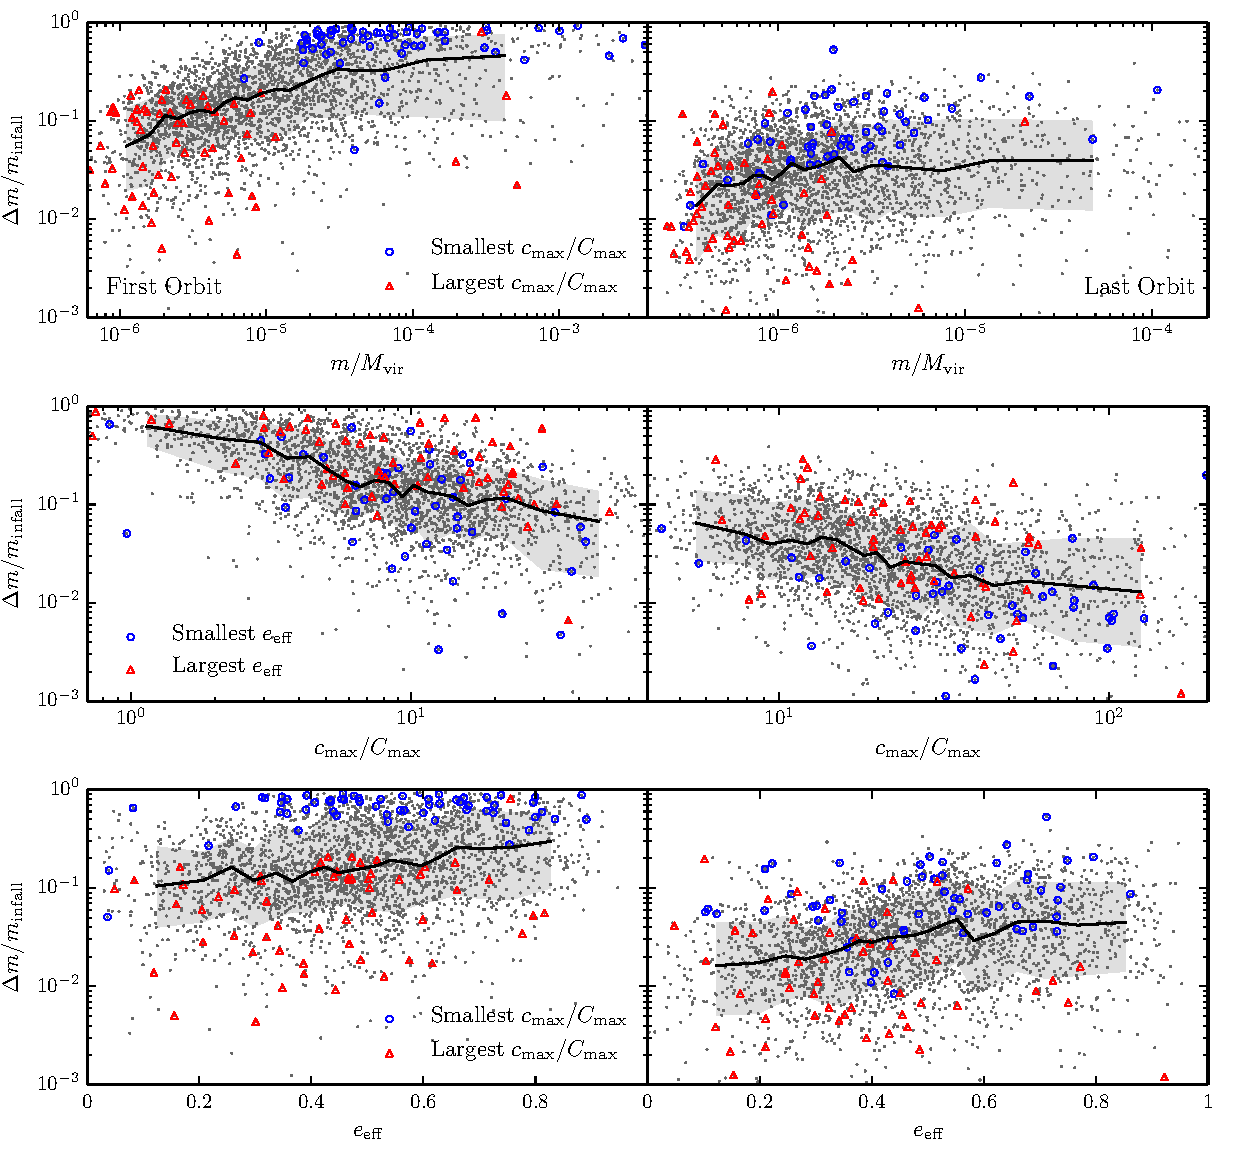
\includegraphics[width=\smwidth]{./figures/neutrinos/fig11.pdf} \vspace{-0.1cm}
\caption[Correlation length as a function of neutrino mass]
{The correlation length defined to be the distance for
which the correlation function in equation (\ref{eq:corrfun}) drops
to half its maximum value for varying neutrino masses.  The
simulations have longer correlation lengths but follow a
similar power law behaviour.}
\vspace{-0.2cm}
\label{fig:corrlength}
\end{center}
\end{figure}
% -------------------------------------------- FIGURE 11 --------------------------------------------

% ================================================================================
% DISCUSSION
% ================================================================================  
  
\section{Discussion}
\label{sec:discussion}
  
We have tested four methods of computing the velocity field: a nearest particle method, a momentum method, and reconstruction via CDM and halo density fields.  Our results are generally consistent with theoretical expectations and highly correlated among each other.  Specifically we have demonstrated that reconstructing the velocity from point-particle halos produces a velocity field highly correlated with that of our $N$-body particles.  It is the near unit correlation coefficient - a measure of the angle between the two fields - that ensures that the reconstructed velocity points in the right direction.  The magnitude of the velocity can then simply be scaled to the correct value as long as the bias is known. 

This result allows for a prescription to determine the actual velocity fields in our own Universe.
\begin{enumerate}
\item Reconstruct the galaxy density field from a galaxy survey catalogue. We expect this reconstruction to be very comparable to the halo reconstruction we use here except with the addition of a 1-halo term to make the bias constant over more wavenumbers.
\item Fourier transform the gridded density field.  Then, use equation (\ref{eq:vrec}) to compute the CDM, neutrino and relative velocity fields in Fourier space.  Here, a nonlinear correction can be applied by additionally multiplying by a factor of $\Delta_v^{\rm Sim}/\Delta_v^{\rm Rec HA}$.
\item Fourier transform back to real space.
\end{enumerate}
We first note that a similar process could be performed on the density fields produced by 21 cm observations.  We also note that redshift distortions and masking effects might result in extra biases in the reconstruction scheme.  We intend to investigate these effects in a future paper. 
  
Our results also provide support for the applicability of the analysis performed in \citet{zhu/etal:2014b,zhu/etal:2014a}.  They used moving background perturbation theory to study the neutrino relative velocity effect.  The moving background approximation relies on having a coherent background relative flow and our simulation results indicate that the coherency scales of such motions are larger than predicted.  Thus, we expect that inaccuracies in the predicted dipole distortion to the correlation function will come from nonlinear evolution rather than the moving background approximation.  We note that we can also directly measure the dipole correlation function in our simulations and plan to report on this in a subsequent paper.  
  
% ================================================================================
% CONCLUSION
% ================================================================================  
  
\section{Conclusion}
\label{sec:conclusion}
  
We performed a set of four large $N$-body simulations including cold dark matter and neutrinos of varying mass.  We have accurately measured the cold dark matter-neutrino relative velocity.  We find that we can accurately reconstruct this velocity using a linear theory approach and halo density fields.  We have described a simple method for accurately predicting the relative velocity field via a galaxy survey or 21 cm observations.  Since such a reconstruction allows for an independent measurement of neutrino masses, we expect this technique to provide significant constraints in upcoming astronomical surveys.  

% ================================================================================
% ACKNOWLEDGEMENTS
% ================================================================================

\section*{\centering Acknowledgements}

We acknowledge valuable discussions with Joel Meyers, Yu Yu and Francisco Villaescusa-Navarro.  We acknowledge the support of NSERC. Computations were performed on the GPC supercomputer at the SciNet HPC Consortium \citep{loken/etal:2010}. SciNet is funded by: the Canada Foundation for Innovation under the auspices of Compute Canada; the Government of Ontario; Ontario Research Fund - Research Excellence; and the University of Toronto.
  

%\include{./sections/frb_modelling}
%\include{./sections/frb_statistics}
% \chapter{Pulse Microstructure}
\label{chapter:microstructure}
\chaptermark{Microstructure}

% \textbf{Think this is the largest set of B0329+54 single pulses 
% studied at $\mu$s. Check. \\ 
% Maybe include gamma arguments P/tms about 1000 for this pulsar 
% seems to be too big for flux tubes \\ 
% bartel \citep{1981A&A....93...85B} observed with 2.5 $\mu s$}

% ================================================================================
% CHAPTER OVERVIEW
% ================================================================================

\section{Chapter Overview}
In this chapter we present results from full-polarization  
single-pulse observations of pulsar B0329+54. 
We have over $10^4$ pulses 
collected with the Algonquin Radio Observatory 46\,m telescope
with 2.56\,$\mu$s time resolution and 390\,kHz 
frequency bins. 
We find microstructure to be a generic broad-band property of 
individual pulses at 400-800\,MHz. 
We also analyze B0329+54's quasi-periodic structure
using a reduced autocorrelation function (rACF). 
Unlike in some pulsars, 
we do not find a single characteristic timescale in its quasi-periodicity, 
although the range of periods is consistent with the known
$t_{\mu} \approx 6 \times 10^{-4} P$ and 
$T_{\mu} \approx 10^{-3} P$ relations. 
Our polarimetry results agree with 
\citet{2015ApJ...806..236M}, in that the periodicity 
of both linear and circular polarization microstructure 
traces closely the total power. 
We also investigate the spectral properties 
of micropulses within a sub-pulse. It is shown that the microstructure not 
only has a wide bandwidth, but that adjacent broad-band 
microstructures can have very different spectra. 

%================================================================================
% INTRODUCTION
% ================================================================================

\section{Introduction}

Within only a few years of the discovery of pulsar B1919+21
in 1967 it had 
become clear that there was great variation between 
individual pulses, and 
even structure within pulses 
\citep{1968Natur.218.1122C, 1975ApJ...196...83M, 1975Natur.257..293R}. 
% Insert citation for this variation.
Each pulsar's folded and integrated profile 
is highly reproducible and specific to that pulsar, 
however the pulses of which they are comprised are 
diverse in a multitude of ways \citep{1998pulsarastronomy}. 
Variation of polarization fraction and mode, intensity 
fluctuations of sub-pulses, and variable arrival times 
are examples of the pulse-to-pulse dynamics. Nulling 
and pulse drifting are also common, and still these 
ostensibly stochastic phenomena result in recognizable 
folded profiles. An example of this is shown in 
Fig.~\ref{fig-pulse_outline}, in data taken at ARO. 

\begin{figure}[!h]
\begin{center}
\includegraphics[trim={0in 0in 0in 0in}, width=1\textwidth]{./figures/microstructure/B0329_average_single.png}
\vspace{0.0cm}
\caption{The average profile of pulsar B0329+54 (dashed, black line)
plotted over a single pulse (solid, maroon line). Though 
there is significant variation from pulse to pulse in 
each of the sub-components (of which there are 
as many as 9 \citep{2001ApJ...555...31G}), 
the average profile is 
well known and repeatable. It can be thought of as a 
probability distribution from which the power in each 
phase bin for a single pulse is drawn.}  
\vspace{-0.4cm}   
\label{fig-pulse_outline}
\end{center}
\end{figure}

Understanding the physical mechanism by which pulsars emit in the 
radio has proven one of the hardest problems 
in modern astrophysics \citep{1975ARA&A..13..511G, 2000ASPC..202..721M}. 
Most of what is known has come 
from folded pulse profiles, but given the substantial 
phenomenology on timescales of individual pulses, there 
is good reason to study them.

On the shortest timescales, microstructure appears in a number of pulsars 
\citep{1975PhDT.........9C, 1982ApJ...254L..35B, 
1998A&A...332..111L, 2002A&A...396..171P}. 
This usually involves 
intensity variation on sub-millisecond timescales. 
They can exhibit periodic oscillatory fluctuations 
as well as broad-band features \citep{1981A&A....93...85B}. 
%\textbf{DESCRIBE IN MORE DETAIL}
Although the phenomenon has been seen in a number of slow pulsars 
at a range of frequencies, there is 
no agreed upon explanation for the origin of microstructure 
\citep{1998A&A...332..111L}. 
\citet{vanhorn} argued the phenomenon was not magnetospheric
but rather a result of neutron star vibrations, 
hence the periodic nature of the substructure. 
Another explanation has been to evoke propagation 
effects in the pulsar magnetosphere. Most commonly, though, 
models for these $\sim$microsecond intensity 
fluctuations have assumed it is fundamentally 
related to the emission mechanism 
rather than a separate process occurring elsewhere 
in the magnetosphere \citep{1998A&A...332..111L}.

Before linking microstructure to broader emission mechanisms, 
it is useful to remind ourselves about the potential 
sources of radio emission in pulsars. 
One prominent explanation is the vacuum curvature 
radiation model. Curvature radiation is similar to 
synchrotron except with a pitch angle that is nearly zero.
In the pulsar magnetosphere, this happens when electrons or positrons 
travel along the very strong curved
magnetic field lines, radiating 
at some critical frequency $\nu_c \sim \gamma^3 c/r_B$, 
where $r_B$ is the radius of curvature of the field lines and 
$\gamma$ is the Lorentz factor
\citep{1998pulsarastronomy}. Given the 
expected relativistic electron-positron plasma over-density at the
pulsar's polar caps and the strong magnetic fields there, 
curvature radiation seems like a natural explanation 
for radio emission. One difficulty with the model is that 
due to the exceedingly high brightness temperatures of 
pulsars, it has always been known that 
coherent emission is needed. For the vacuum curvature 
scenario, this requires ``charged bunches" of electrons 
($\sim$10$^{15}$ particles) emitting coherent curvature radiation 
\citep{2004ApJ...600..872G}, and it is not obvious 
how these bunches would be created.

The single-particle vacuum curvature-radiation model 
can be informed by observations microstructure and 
its polarization. Since the sub-pulses that make 
up individual pulses can be further broken down into 
microstructures, those microbursts should show phenomena 
predicted by thoery. The consequences of 
an incoherent sum of charged bunches 
emitting coherent curvature radiation can be found 
in \citet{1990A&A...234..269G} and summarized 
in \citet{2015ApJ...806..236M}.

Few detailed polarization studies of 
microstructure have been carried out. 
\citet{1978A&A....64...27F} commented on the qualitative 
polarization properties of microstructure seen in B1133+16. 
\citet{2002MNRAS.334..523K} quantitatively analyzed polarimetry 
observations of Vela's microstructure. Recently, however, 
\citet{2015ApJ...806..236M} made a convincing case for 
studying short-timescale 
fluctuations of polarized pulsar emission. 
They observed almost three 
dozen sources with $\sim$60\,$\mu$s time-resolution at 
Arecibo with periods ranging from 0.15-3.7 seconds.



% ================================================================================
% THEORY AND IMPLEMENTATION
% ================================================================================

\section{B0329+54 Individual Pulses}

\subsection{Observations}

The data for our B0329+54 single-pulse analysis 
were taken at the Algonquin Radio Observatory (ARO). 
The refurbished 46\,m antenna was mounted with a 400-800\,MHz 
CHIME four-leaf clover feed, the details 
of which are described in Chapter \ref{chapter:chime}. 
We attached to it a custom back-end 
made from CHIME hardware and software that can write voltage 
data to disk with $\sim$390\,kHz spectral resolution 
and 2.56\,$\mu$s temporal resolution. We refer to this as ``baseband". 
Though the data is channelized with a polyphase filter bank (PFB),
the process is invertible and we are able to 
de-channelize in order to coherently dedisperse offline. Data are written 
in the VDIF specification, similar to the Pathfinder data format 
described in Chapter \ref{chapter:beamforming}. However in 
the case of ARO, since we have 2 channels instead of 256, we do 
not need 16 FPGA boards and 16 GPU nodes to process the data. 
Therefore frequencies need not be reassembled because 
each frame contains all 1024 contiguous frequencies. There 
are also slight changes to the header. 
We observed the pulsar for roughly 2 hours on 1 August 
2014, for more than 10$^4$ pulses. 


\subsection{Data post-processing}
\label{sec-b0329analysis}

We use a VLBI pulsar analysis code-base called 
{\tt scintellometry}, which was built for 
correlating baseband data from different telescopes 
with differing data formats\footnote{https://github.com/mhvk/scintellometry}. 
Though the code is able to coherently dedisperse, 
B0329+54 is slow and has a DM of only 
$\sim$27 pc cm$^{-3}$, and we have found it is sufficient to do ``by-channel" 
dedispersion. This means stepping through each frequency 
of the channelized voltage data, inverse Fourier transforming 
that frequency's time series, and dedispersing that up-channelized 
chunk. The resultant DM-smearing in the case of 
B0329+54 is negligible. 

The two dedispersed voltage time-streams are then correlated, 
providing four real numbers per time and frequency. 
Out of these correlations the Stokes parameters 
can be constructed. The four numbers are an autocorrelation for each 
polarization, and the real and imaginary components of the
cross-correlation. The output array is therefore,

\begin{equation}
D = \begin{pmatrix}
\left< X_0X_0^*\right> & \left< \Re e\{X_0X_1^*\}\right >\\ 
 \left< \Im m\{X_0X_1^*\}\right > & \left< X_1X_1^*\right>
\end{pmatrix}.
\end{equation}
\\
\noindent By rearranging these, the Stokes parameters can 
be obtained as follows,
\\
\begin{equation}
\begin{pmatrix}
\left< X_0X_0^*\right> & \left< X_0X_1^*\right >\\ 
 \left< X_0^*X_1 \right > & \left< X_1X_1^*\right>
\end{pmatrix} = 
\begin{pmatrix}
I + Q & U + iV\\ 
U -iV & I - Q
\end{pmatrix}.
\end{equation}


\noindent These intensities are either folded 
or written to a dedispersed time and frequency {\tt numpy} 
array with arbitrary time rebinning. 

Before the polarization data can be analyzed, 
we must remove two effects. The first is the 
sinusoidal phase in frequency introduced by cable delays. 
This comes from that fact that the two polarizations signals, 
$X_0$ and $X_1$, end up with slightly different instrumental 
phases due to things like disparate cable lengths. When 
the signals are correlated, a constant phase offset (time lag) 
becomes a sinusoidal oscillation in frequency. 
Written in terms of the Stokes parameters
this transformation takes,

\begin{equation}
X_0 X_1^* = U + iV,
\end{equation}

\noindent and makes the cross-pol correlation

\begin{equation}
X_0 X_1^* \rightarrow \left (U + iV \right) \times e^{2\pi i \nu \tau},
\end{equation}

\noindent where $\tau$ is the instrumental time lag
between the two polarizations. This rotates Stokes V 
into Stokes U, thereby leaking circular into linear polarization.

Another effect is Faraday rotation, which is significant 
for B0329+54 in our band. Its RM is $\sim$64\,rad\,m$^{-2}$, 
resulting in several phase wraps between 400-800\,MHz.
Unlike cable delays, the Faraday effect rotates the 
linear polarization vector, $P_L$, defined by:

\begin{equation}
P_L \equiv Q + iU.
\end{equation}

\noindent Similar to dispersion, it depends on $\lambda^2$.
The linear polarization is rotated as,

\begin{equation}
P_L \rightarrow P_L\, e^{2i\, \textrm{RM} \, \lambda^2}.
\end{equation}

We remove these two effects by doing a joint fit 
of the folded pulse profile at each frequency. We fit 
for time lag, $\tau$, $\rm RM$, Stokes 
Q, U, and V, as well as global phase offset, $\phi_{X_0,X_1}$. 
Though we do not do a full polarization calibration of 
the ARO feed, we have verified that its leakage is 
not too severe. This was done by measuring pulsar 
B1929+10, whose polarization angle swings by $\sim$80 
degrees in a known way, and comparing our results to a
calibrated template in the literature. We found 
small deviations from the known template of 
less than $\sim$5$\%$ in slope.

corr-vdif burst-search network

\section{Microstructure}

The polarization and 
total intensity of B0329+54 vary on a range of scales. 
Though the polarization in its folded profile is less than 
10$\%$ for both linear and circular, the 
mode and fraction from individual pulses 
jumps around. The pol-fraction for single pulses 
can surpass $70\%$. The total intensity is modulated 
at a number of different locations.
In the ISM, scintillation causes the pulsar's brightness to fluctuate 
on timescales of 5-30 minutes. Between individual pulses there is  
variation by factors of a few, which is presumably intrinsic 
to the source. Within a pulse (timescales $\lesssim 50$\,ms), 
brightness changes exist due to the multi-component nature 
of B0329's pulse profile. Finally, 
we see sub-millisecond fluctuations within these sub-pulses, 
which are the subject of this chapter.
Fig.~\ref{fig-alltscales} shows such variation on 
minutes, seconds, and millisecond timescales respectively,
going from top to bottom.

\begin{figure}[!h]
\begin{center}
\includegraphics[trim={1.5in 0in 1.5in 0in}, width=\textwidth]{./figures/microstructure/allscales.jpeg}
\caption{Pulsar B0329+54 intensity fluctuations 
on three different timescales. From top to bottom panel: roughly 
2,500 pulses over a half hour; pulse-to-pulse brightness 
variation; and intra-pulse variation on timescales of 50\,$\mu$s-10\,ms.}
\vspace{-0.75cm}   
\label{fig-alltscales}
\end{center}
\end{figure} 

\subsection{Quasi-periodicity}

Several pulsars are known to exhibit quasi-periodic 
trains of micropulses. \citet{1990AJ....100.1882C} 
found periodic variation in pulsars 0809+74, 0950+08, 
1133+16, 1944+17, and 2016+28. They found that each 
source's microstructure had a characteristic quasi-period, 
and that for some pulsars the strength of microstructure 
scaled inversely with frequency. 

In B0950+08, the periodic microstructure 
looks similar to Crab ``nanoshots".
The flux between micropulses almost entirely disappears 
and the bursts themselves are incredibly narrow ($\lesssim$10\,$\mu$s)
\citep{2002ARep...46..206P}. 
In B0329+54 we see quasi-periodic structures in a 
number of our strong pulses. However unlike in B0950 or 
the Crab, it seems to be a component that sits on 
top of an underlying smooth profile. To determine the 
timescales of this quasi-periodicity, we compute 
a reduced autocorrelation function (rACF). ACFs
have long been used to study microstructure
\citep[see][]{1978AZh....55.1024K, 1998A&A...332..111L}. 
It is computed as,

\begin{equation}
A(\tau) \equiv \frac{\int S(t)S(t + \tau) \, \textrm{d}t}{\int S^2(t)
\, \textrm{d}t},
\end{equation}

\noindent where $S(t)$ is any time-stream intensity, 
whether Stokes I, Q, U, or V. 
The maxima, minima, and slope changes of $A(\tau)$ 
can inform us about relevant timescales in the pulse
\citep{2015ApJ...806..236M}. 

For pulsars like B0329+54 whose microstructure often 
sits on top of a smoother pulse profile, $A(\tau)$
does not exhibit obvious structure. To avoid this problem 
we fit each sub-pulse with a Gaussian, subtract 
that off, then calculate the ``reduced" ACF using,

\begin{equation}
S'(t) \rightarrow S(t) - \mathcal{N}(\mu_{\rm fit}, \sigma^2_{\rm fit}).
\end{equation}


\begin{figure}[!h]
\vspace{-0.1cm}
\begin{center}
\includegraphics[trim={2in 1in 2in 0in}, width=\textwidth]{./figures/microstructure/quasi_periodicity.jpeg}
\vspace{0.4cm}
\caption{Periodicity and quasi-periodicity seen in 
     microstructure from 
     two different B0329+54 pulses, but on the same sub-pulse. 
     The top left panel shows a pulse with a periodic train of microbursts
     for both the raw profile (slate blue) and the 
     Gaussian-subtracted profile (black). The bottom 
     left panel shows broader and more modulated 
     quasi-periodic microstructure. The right panels 
     show the corresponding ACF (slate blue) and rACF (black).
     }
\label{fig-quasistruct}
\end{center}
\end{figure}

An example of this is 
shown in the Fig.~\ref{fig-quasistruct}. The left 
panels shows bright single pulses with a
trains of microbursts for both $S(t)$ and $S'(t)$.
The right panel shows the corresponding ACFs. The 
black curve is the rACF, since it is 
the autocorrelation of a Gaussian-subtracted pulse. 
There are two striking features about these plots. The first 
is that unlike other pulsars that exhibit microstructure,
B0329+54 does not seem to have a characteristic period or width 
to its structure. This is seen by comparing the first 
minima and maxima of the correlation functions and 
noticing they are at different timescales for the two 
pulses. The second is that the correlation function 
contains very little information if a smooth 
component is not first subtracted, i.e., if 
the rACF is not computed.

There is a known correlation between microstructure 
timescales and the pulsar period. 
\citet{2002MNRAS.334..523K} have shown the scaling to be,

\begin{equation}
t_\mu \approx 6\times10^{-4} P,
\end{equation}

\noindent where $P$ is the pulsar's period and 
$t_\mu$ is the timescale of individual microbursts, 
often estimated by the first local minimum in the ACF. 
This was consistent with the original claim by 
\citet{1979ApJ...233..981C}. 
\citet{2015ApJ...806..236M} used 24 L-band pulsars 
to revisit the relationship. Instead of using $t_\mu$, 
they used the period of quasi-periodic microstructure, 
$T_\mu$, and found it too increased 
with pulsar period as $\sim 10^{-3} P$. Here we will follow suit and 
focus primarily on the first local maximum. The reason we use
this rather than widths of individual microbursts 
is because those are often unresolved in time or scattered 
by the ISM. 

For B0329+54 we find the absence of a characteristic 
timescale, but consistency with 
the known $t_\mu-$ and $T_\mu-P$ relation. 
In Fig.~\ref{fig-quasistruct} we show 
an illustrative example of the differences in 
microstructure timescales from pulse to pulse. The 
top row's pulse has $t_\mu \sim 0.28$\,ms and 
$T_\mu \sim 0.55$\,ms, whereas the bottom row's pulse 
has $t_\mu \sim 0.68$\,ms and $T_\mu \sim 1.2$\,ms.
For B0329+54 we expect the first minima of rACFs
to be around $400$\,$\mu$s and the first maxima 
to be at $700$\,$\mu$s. In general, we find a range of 
$t_\mu \sim 100-1000$\,$\mu$s and 
$T_\mu \sim 500-2000$\,$\mu$s, which are consistent 
with the trend seen in other pulsars. 

There are two basic ways to get sub-millisecond 
variations in pulsars: angular beaming in the 
direction transverse to the observer, and actual temporal 
modulation in the magnetosphere.  
To interpret our measured timescales, we can start 
in the framework of a beaming model, in which 
the width of a micropulse is given by a 
radiating point source with some Lorentz factor, $\gamma$.
If we take $t_\mu$ as an upper limit for the 
width of a microburst, the pulse's width in radians is 
at most,

\begin{equation}
\phi = 2 \pi \, t_\mu / P\,.
\end{equation}

\noindent The Lorentz factor will be given by,

\begin{equation}
\gamma = \frac{1}{\phi\, \textrm{sin}\delta}\,,
\end{equation}

\noindent where $\delta$ is the angle between 
the pulsar's rotation axis and the line of site \citep{1998A&A...332..111L}.
Our results give a lower-limit on $\gamma$ of 
$\sim$500-1200. This is difficult to reconcile 
with several theoretical studies, which suggest 
the particles producing microstructure should have
$\gamma<100$ \citep{1992msem.coll..322A, 1998A&A...332..111L}.

In the temporal modulation picture, the effect
is not geometric but due to fluctuations in 
the intensity of waves propagating in the magnetosphere.
\citet{1983Ap&SS..97....9C} is an example of a temporal model, which 
does not require any beaming. In it, non-linear effects 
in the polar-cap plasma lead to intensity modulation 
along the radial direction.

\subsubsection{Polarized periodicity}

\citet{2015ApJ...806..236M} found that not only did 
their set of low-Galactic latitude pulsars 
have characteristic periodicities ($T_\mu$), but that 
those timescales were common across all Stokes 
parameters. Though we do not find a repeatable 
timescale in B0329+54, we do find its 
quasi-periodic microstructure to have the same 
timescales in Stokes I, V, and linear polarization.
We can see this visually 
for I and $|P_L|$ in Fig.~\ref{fig-polwaterfall}.

\citet{2015ApJ...806..236M} suggest that the similarity of 
the microstructure in 
linear and circular polarization with total intensity 
means the structures cannot be 
caused by coherent curvature radiation. 
\citet{1990A&A...234..269G} worked through the 
polarization consequences of a model 
in which the incoherent superposition of a large 
collection of sub-nanosecond pulses produced 
by the curvature mechanism resulted in pulsar radio emission.
They found the charged bunches in vacua scenario predicts
sign-changing circular polarization. Since 
\citet{2015ApJ...806..236M} do not see 
handedness switching in individual microbursts, they conclude 
that such a mechanism cannot be the source of microstructure.  
We looked for a similar effect. In sub-pulses that had both significant 
Stokes V and modulated microstructure we did not find any sign-changes, 
even when the circular polarization went from right- to left-handed
across the sub-pulse. A caveat is that we do not find any 
microstructure as heavily modulated or resolved as the pulses 
\citet{2015ApJ...806..236M} found, meaning the microbursts 
we observe could be de-polarized or the sum of multiple 
modes. Therefore we do not claim that the 
absence of a sign change in B0329+54's microstructure 
can definitively rule out charged bunches emitting 
curvature radiation as their source. Instead we simply note 
that this feature was not seen, and might have been seen 
in the coherent curvature radiation model.


\begin{figure}[!h]
\vspace{-0.1cm}
\begin{center}
\includegraphics[trim={0in 0in 0in 0in}, width=\textwidth]{./figures/microstructure/micro_pol_waterfall.png}
\caption{An example of the way the linear polarization 
     traces periodic microstructure.}
\label{fig-polwaterfall}
\end{center}
\end{figure}

\subsection{Microburst spectral variation}

In some of the brightest pulses we find frequency 
variation between individual microbursts. Given 
the timescales invovled (200-1500\,$\mu$s), such 
variation is not expected to be due to propagation 
effects like scintillation. The top right panel of 
Fig.~\ref{fig-spectralvar} shows the same pulse at 
450\,MHz (red) and 640\,MHz (black). We isolate the
three brightest individual micropulses shaded by 
light blue, light red, and grey. One can see the 
light blue pulse is quite bright at 640\,MHz, 
but less so at 450\,MHz. The light grey pulse almost 
completely disappears by 640\,MHz, even though 
it is prominent at lower frequencies. The light 
red microburst is somewhere between the other two.

In order to 
compare the frequency structure more easily, the off-pulse 
(any RFI or Galaxy in the beam) was subtracted, and the 
averaged pulse profile of B0329+54 was divided out.
This is why the spectra in the bottom panel of Fig.~\ref{fig-spectralvar}
are nearly flat. 

The difference in spectral behaviour for 
adjacent micropulses is difficult to explain 
if microstructure is caused by temporal 
variation in the magnetosphere. If each pulse is not a result 
of an individual collection of coherently emitting 
charged bunches, then why would frequency behaviour 
changed so drastically on such a short timescale?

\begin{figure}[!h]
\vspace{-0.5cm}
\begin{center}
\includegraphics[trim={1.8in 0in 1.in 0in}, width=\textwidth]{./figures/microstructure/spectra.jpeg}
\caption{An example of broad-band microstructure in a 
particularly bright pulse. This pulse's three most prominent 
microbursts have very different frequency behaviour. \textit{top left:}
Frequency time colour map showing this pulse over the 
full band, for roughly 15 ms. The broad-band nature of 
the microstructure is also apparent as 
vertical pipe-like structures. \textit{top right:} Pulse 
profile for two different frequencies: centered on 640\,MHz and 450\,MHz, 
averaged over $\sim$40\,MHz. The three vertical shaded regions, 
blue, red, and grey, correspond to the three brightest 
micropulses, ``micropulse 1", ``micropulse 2", ``micropulse 3", 
respectively. One can also see their differences in their 
spectral behaviour. The first spike is brighter at 450\,MHz
than at 640\,MHz, but the opposite is true of the
second and third spikes. \textit{bottom panel:} The relative 
spectra of three micropulses, with colours corresponding 
to the shaded region in the top right panel.}
\label{fig-spectralvar}
\end{center}
\end{figure}

% \subsection{Microstructure and DM}
% Variation in DM leads to significant uncertainty in pulse
% time-of-arrival (TOA). Folded spectra from slow 
% pulsars provide a profile that is 
% too broad to precisely measure DM. Microstructure, on
% the other hand, can be as narrow as pulses from 
% millisecond pulsars (MSPs).


% \begin{figure}[!h]
% \begin{center}
% \includegraphics[trim={0.in 0in 0.in 0in}, width=\textwidth]{./figures/microstructure/DM_from_folded_pulse.png}
% \vspace{0.0cm}
% \caption{}
% \label{fig-micro}
% \end{center}
% \end{figure}



\section{Conclusion}
\label{sec:conclusion}
  
We have presented analysis of the largest collection 
of single-pulse microstructure data of 
B0329+54. Broadband microstructure was found to be a 
generic property of this pulsar, although it is
rarely highly modulated. The sub-pulses we analyzed often 
exhibited quasi-periodic trains of micropulses. We 
quantified such periodicity with a reduced autocorrelation 
function, which pulls out time-like correlations by 
first removing the stronger, smooth component of the 
sub-pulse. The quasi-periodic microstructure of B0329+54
were found to have no single characteristic timescale, which is
different from other pulsars that have been studied. 
However, we did show that the range of periods are 
consistent with the known $T_\mu \approx 10^{-3}\,P$ relation. 
The micropulse widths are also roughly consistent with 
the known $t_\mu-P$ scaling. These scalings held for 
the polarized microstructure as well. Linear polarization 
and Stokes V were both found to mimic total intensity in 
their quasi-periodicities. As \citet{2015ApJ...806..236M} 
have shown, one would not necessarily expect this 
if the microstructure came from 
coherent curvature radiation of charged bunches in a vacuum.

The microburst widths allowed us to estimate the Lorentz 
factor of the radiating particles, assuming the widths 
are due to relativistic beaming. We find $\gamma\sim500$-$1200$, 
which are higher than the expected particle velocities. 
This inconsistency was also found by \citet{1998A&A...332..111L}, 
who use it to reject the beaming model. The other standard 
explanation for the origin of pulsar microstructure is not 
geometric but temporal. The idea is that time-like 
fluctuations in the magnetospheric plasma generate the 
periodic and quasi-periodic trains of sub-millisecond pulses
that are observed in a number of sources. 

In the framework of this model, we found the spectral 
behaviour of B0329+54's microstructure to be difficult
to interpret, though we do not claim to 
rule it out. In several strong pulses we found 
micropulses within a single sub-pulse to have very different 
broad-band frequency characteristics. If the pulses 
do not come from physically separate collections of 
charges, then we would not naively expect vastly different 
spectral properties. That said, theoretical work must be 
done to address the polarization and spectral features of 
a temporally modulated plasma in the emission region 
before strong claims can be made.





%\include{./sections/conclusions}

% ==============================================================================
% BIBLIOGRAPHY
% ==============================================================================

\addcontentsline{toc}{chapter}{Bibliography} % Adds a line for the Bibliography in the Table of Contents.

\bibliographystyle{apj}
\bibliography{references}

\end{document}
